% ============================================================
% Materials and methods
% ============================================================

\subsection{Overview and evidence-integration strategy}
\label{subsec:workflow-overview}

The analysis combined independent evidence layers rather than treating any
single program as an orthology test. Juvenile skeletal and growth-plate
expression was used to prioritize biologically relevant small leucine-rich
proteoglycans (SLRPs). Candidate proteins were then evaluated by reciprocal
protein similarity, length and annotation checks, Pfam domain architecture,
signal-peptide prediction, multiple-sequence alignment, phylogenetic placement,
protein-language-model embeddings, conserved genomic neighbourhood, and
representative coding-gene structure. Conflicting or incomplete cases were
retained as tentative or excluded only after manual review of the combined
evidence. Exploratory protein-motif, promoter-motif, and phenotype-database
analyses were performed as supplementary validation; they were not used as
stand-alone candidate-selection criteria. The complete decision workflow is
summarized in Figure~\ref{fig:workflow-overview}.

\begin{figure}[htbp]
    \centering
    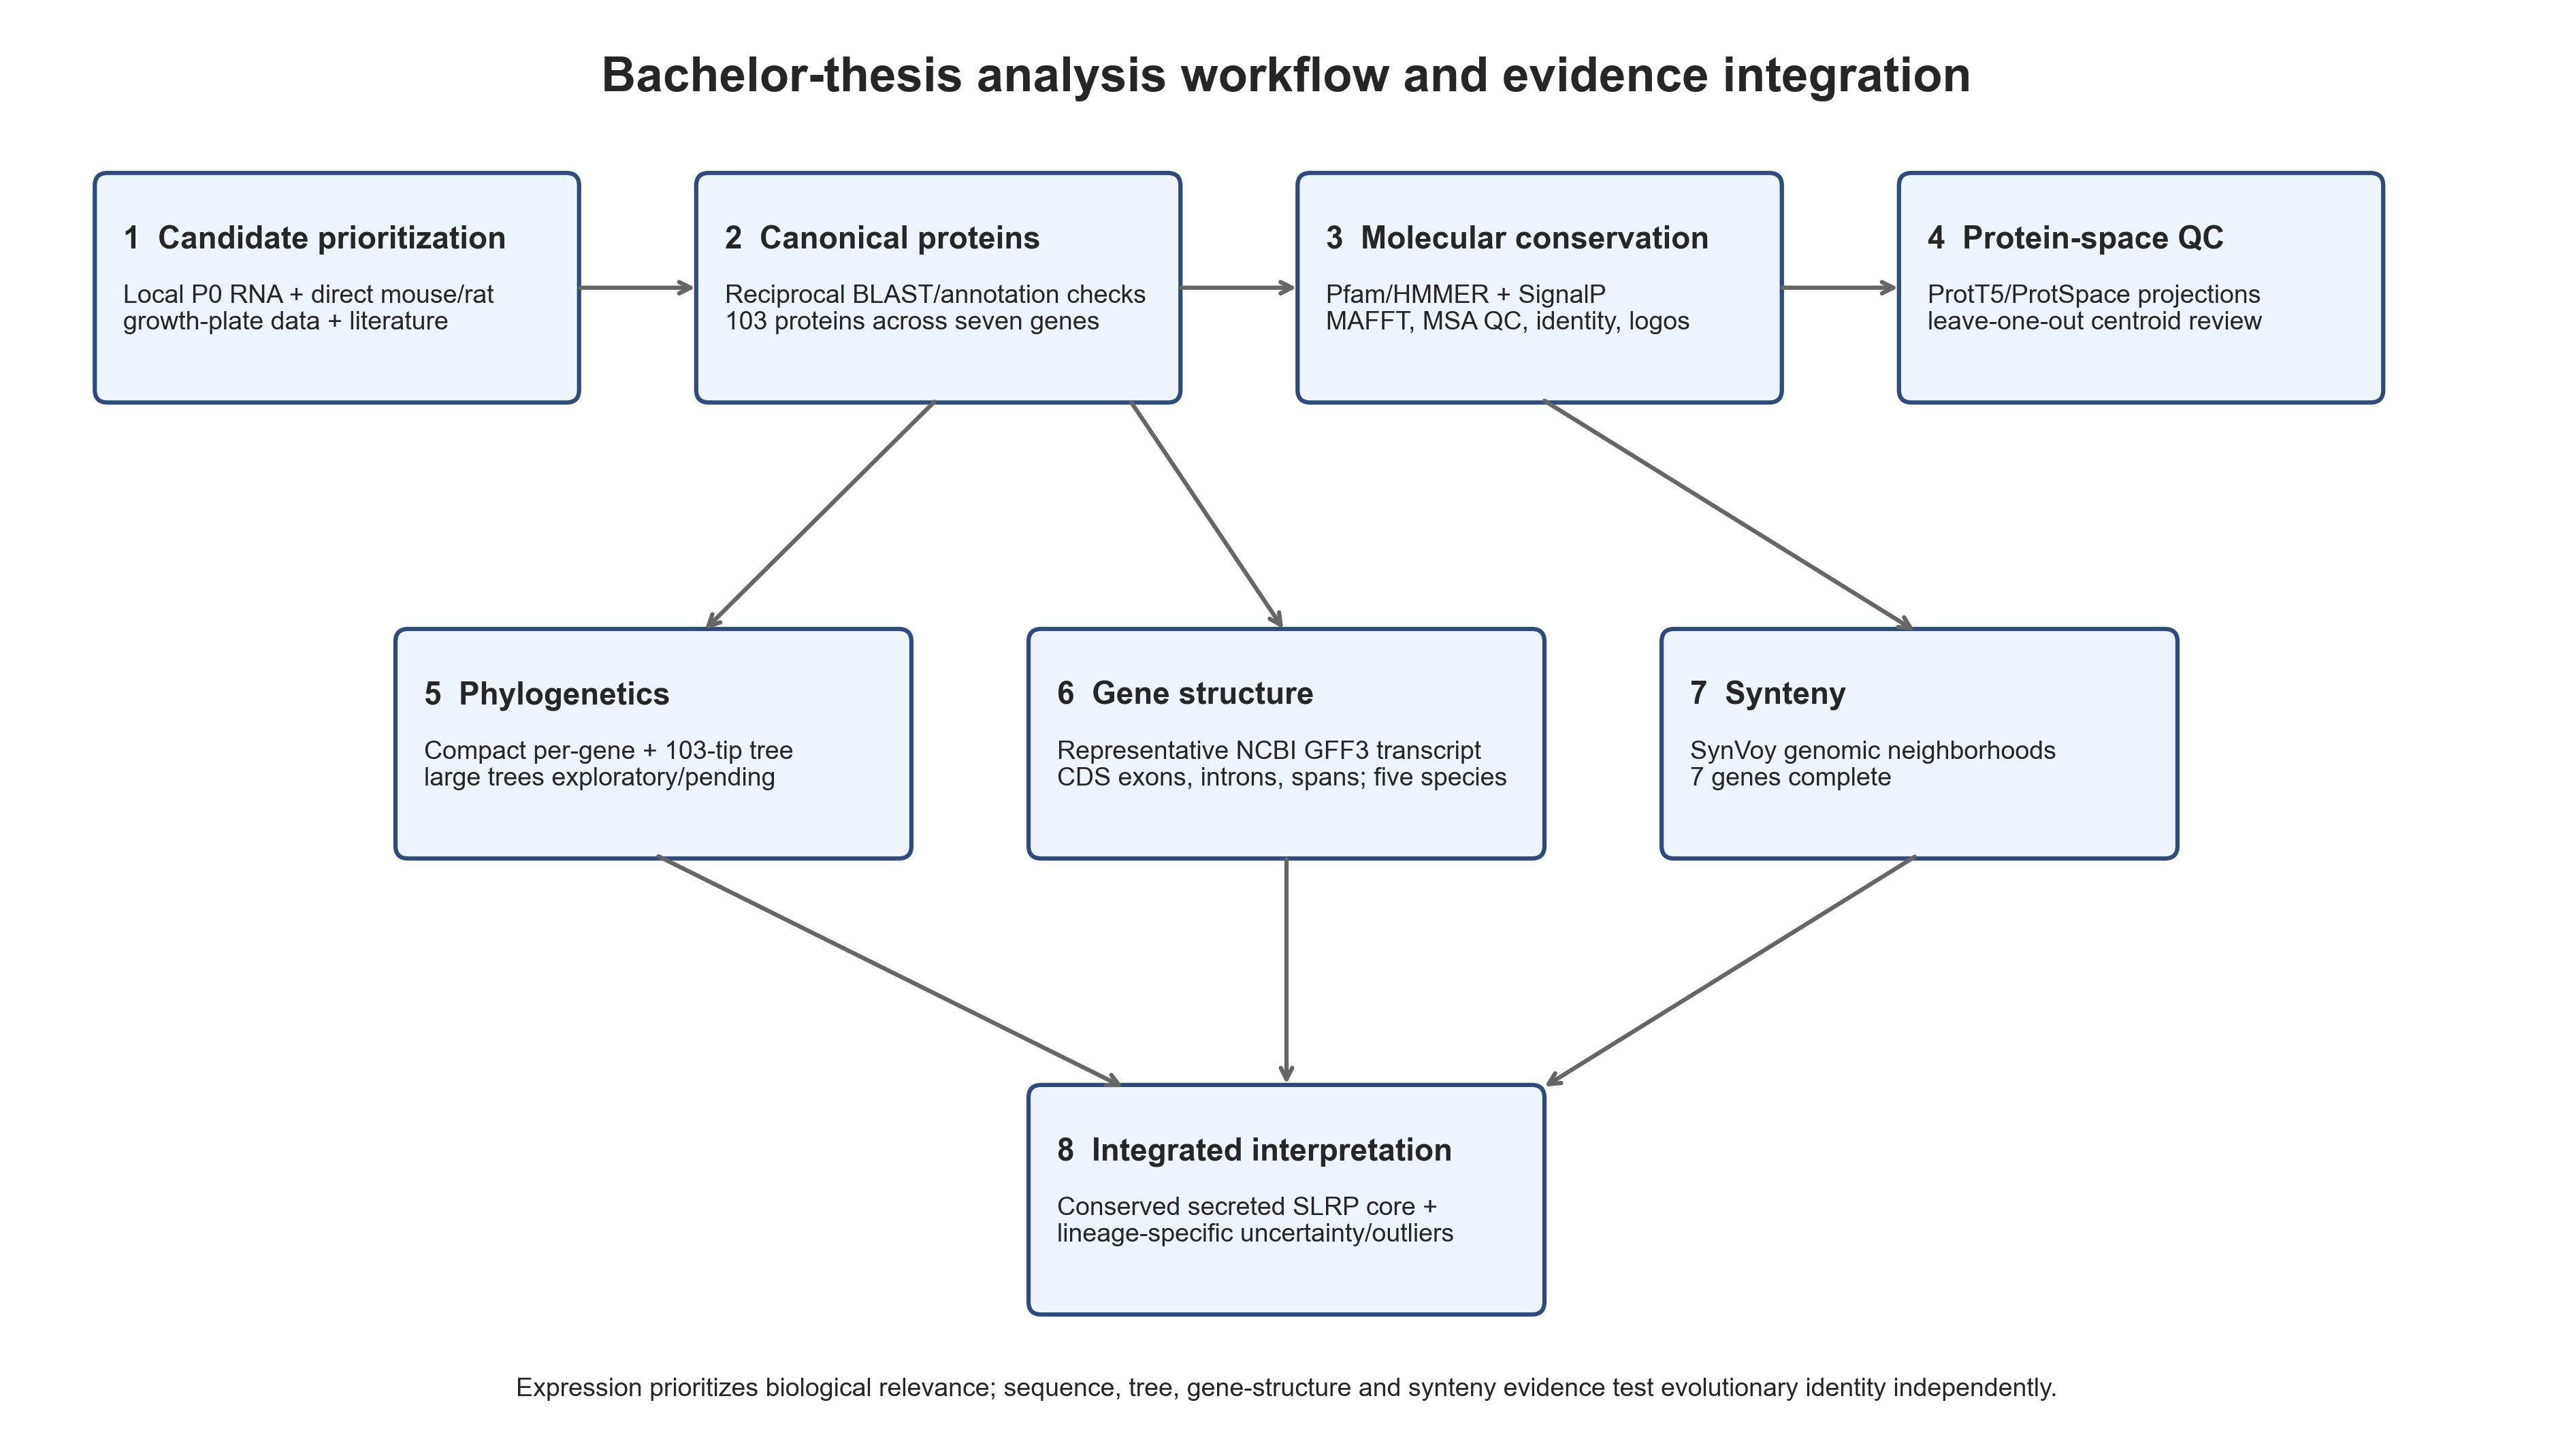
\includegraphics[width=\textwidth,height=0.76\textheight,keepaspectratio]
        {figures/overview/thesis_workflow_overview.png}
    \caption{Overview of the thesis workflow. Expression and literature define
    the biological candidate panel; reciprocal protein searches, domain and
    signal-peptide annotation, alignment, phylogeny, microsynteny, gene
    structure, and manual review provide complementary evidence for ortholog
    plausibility and conservation. Exploratory motif, promoter, embedding, and
    phenotype analyses provide supporting context rather than a single combined
    score.}
    \label{fig:workflow-overview}
\end{figure}

\subsection{Expression datasets and candidate selection}
\label{subsec:rnaseq-expression}

The initial screen used three wild-type samples from the public NCBI Gene
Expression Omnibus study GSE305415 (BioProject PRJNA1305489; raw reads in
NCBI SRA; \url{https://www.ncbi.nlm.nih.gov/geo/query/acc.cgi?acc=GSE305415}).
The selected runs were SRR34978216, SRR34978215, and SRR34978214. The study
obtained Prx1-lineage chondroprogenitors by fluorescence-activated sorting of
digested postnatal-day-0 mouse knee joints \citep{John2026}. The GEO series
description implies RNA extraction after sorting, whereas the individual WT
sample records describe culture toward mature chondrocytes before extraction.
Because this cell-state discrepancy could not be resolved from the deposited
metadata, these samples were treated as P0-derived chondrocyte-lineage material,
not as freshly isolated growth-plate cells. WT1 and WT2 had paired-end runs;
the SRA/ENA run metadata identify WT3 (SRR34978214) as single-end despite the
generic paired-end processing text copied into its GEO sample record.
Previously generated Salmon
\texttt{quant.sf} files stored on the computer were
used because their mapping rates were 81.9--92.0\% and re-extraction reproduced
the previously curated tables. For each sample, transcript TPM values assigned
to the same gene symbol were summed, and the mean, sample standard deviation,
coefficient of variation, and rank of
nine screened SLRPs were calculated across the three wild-type samples. The
original Salmon version and index-building command were not recoverable from the
preserved files; therefore, the analysis is reproducible from the archived
quantifications onward, but this unknown is reported rather than reconstructed.

Four locally available samples from the unrelated ageing atlas PRJNA936435 were
retained only as a descriptive metadata audit. They differed in study, age,
tissue, and replication and were not used for differential expression or for a
growth-plate-versus-other-tissue ratio.

Independent anatomical validation used the processed matrices deposited with
GSE114919. These data contain laser-capture-microdissected proliferative and
hypertrophic zones from mouse and rat growth plates, including tibia at one and
four weeks with five replicates per tibial condition. The authors' normalized
values were retained on their deposited scales. Detection and within-condition
ranks were summarized; values were not pooled with the GSE305415-derived Salmon
TPMs or compared as absolute measurements between species. Bgee 16 expression
calls for mouse, chicken, and zebrafish were used as qualitative context because anatomy,
developmental stage, and assay coverage were not matched among species. Missing
Bgee calls were treated as missing evidence rather than absence of expression.

The final panel was selected from the joint evidence rather than RNA abundance
alone. Selection considered reproducible juvenile expression, direct
growth-plate or cartilage evidence, published skeletal/ECM function, coverage of
SLRP classes I--III, and feasibility of cross-species ortholog analysis. BGN,
DCN, FMOD, PRELP, EPYC, LUM, and OGN were advanced through the full comparative
workflow. DCN also served as the closest paralog control for BGN, and OMD as a
gene-structure and biological-context gene. OGN was designated exploratory
because its growth-plate expression evidence was less consistent. ASPN was kept
as class-I background rather than taken through the full pipeline because its
independent tibial growth-plate support was weaker and less consistent across
the two rodent species, while BGN and DCN already provided the principal
class-I candidate and paralog-control comparison.

\subsection{Reference proteins, ortholog candidates, and manual curation}
\label{subsec:ortholog-search-filtering}

Human proteins served as the query/reference anchors. Candidate proteins were
obtained from NCBI/RefSeq proteomes for a broad chordate panel representing
mammals, bird, reptile, amphibian, teleost and non-teleost bony fish,
cartilaginous fish, jawless vertebrate, and amphioxus comparisons. BLASTP
(version 2.12.0+) was run with an E-value threshold of $10^{-5}$, and reciprocal
searches against the human reference set were used to test gene assignment.
Candidates were screened for compatible annotation, query coverage, protein
length, obvious truncation, and duplicate use of the same accession. A median
length-ratio interval of 0.7--1.3 was used as an automated first-pass filter,
with biologically plausible exceptions assessed manually rather than rejected
solely by length.

The final canonical FASTA contained one nonredundant curated panel per gene.
Manual review in AliView/Jalview emphasized intact N- and C-terminal regions,
conserved cysteine positions, continuous alignment through the LRR-rich region,
absence of large candidate-specific insertions or deletions, and agreement with
reciprocal-hit, phylogenetic, synteny, and SignalP evidence. Exact terminal
identity was not required. Decisions and excluded provenance records were
preserved in the candidate-level confidence table.

\subsection{Domain architecture and signal peptides}
\label{subsec:domain-signalp}

The 103 canonical proteins were scanned with HMMER 3.4 \texttt{hmmscan} against
Pfam-A. Domain hits with independent E-values $\leq 10^{-3}$ were retained, and
LRR/SLRP-family profiles were summarized for each protein. Because related SLRPs
share LRR profiles, this analysis was interpreted as family-membership and
protein-completeness evidence, not gene-specific proof.

Classical secretion signals were predicted with SignalP 6.0 using the eukaryotic
slow-sequential mode. An initial set of 86 retained calls was supplemented by a
final 17-sequence run (job \texttt{6AA7E4B90014723A58E1A86B}), giving predictions
for all 103 canonical proteins (100 positive and three negative). A positive
N-terminal signal is compatible with entry into the
secretory pathway and the expected extracellular localization of SLRPs, but was
not treated as an independent demonstration of in-vivo localization.

\subsection{Multiple-sequence alignment and protein conservation}
\label{subsec:multiple-sequence-alignment}

One alignment per gene was produced with MAFFT 7.505 using
\texttt{--auto}. Pairwise identity was calculated over residue pairs aligned in
both sequences. Per-column occupancy, modal-residue conservation, majority
consensus sequences, species-by-species identity matrices, and sequence logos
were generated from the untrimmed alignments. Untrimmed alignments were retained
for manual biological interpretation so that variable termini and gap-rich
regions remained visible. trimAl 1.5 with \texttt{-automated1} was used to
prepare the combined alignment for phylogenetic analysis.

\subsection{Phylogenetic and embedding analyses}
\label{subsec:phylogenetic-analysis}

Maximum-likelihood phylogenies were inferred with IQ-TREE 2.0.7. ModelFinder
selected the amino-acid substitution model by information criterion
(\texttt{-m MFP}); branch support was estimated with 1,000 SH-aLRT replicates
and 1,000 ultrafast-bootstrap replicates, using automatic thread allocation.
Seven compact per-gene trees were inferred from the canonical MAFFT alignments.
The combined family tree was inferred from the trimAl-filtered 103-protein
alignment. Trees were exported with gene and taxonomic annotation files for
iTOL. Unless an explicit outgroup was applied, trees were interpreted as
unrooted; split support was used for assignment quality and not to infer the
direction or timing of evolution.

As an alignment-independent exploratory check, ProtT5 embeddings were analysed
with ProtSpace projections using PCA, UMAP, and t-SNE. A leave-one-out nearest
gene-centroid test in the original embedding space was used to identify
candidate outliers. Two-dimensional proximity and centroid assignment were
treated as quality-control evidence only.

\subsection{Synteny analysis and manual locus review}
\label{subsec:synteny-analysis}

SynVoy compared the human query locus with 14 non-human target genomes using
the corresponding genome and GFF3 annotation files. Human was therefore the
home-locus anchor rather than an omitted comparison species. The tool's HIGH
and MEDIUM gene-of-interest candidates were parsed after coordinate-ownership
and explicit paralog filtering. Counts refer to retained annotations/candidates,
not a count of proven orthologs. Candidate loci were assigned to P1 detailed,
P2 rapid, or P3 control review according to missing calls, rescue/partial calls,
self-consistency flags, and disagreement with protein or tree evidence.

Runs used protein mode and ten flanking genes. The completed updated-tool BGN
and DCN analyses used MMseqs sensitivity 9.5, non-strict gene-family token
matching, disabled automatic generic presets, an 8-GB MMseqs split-memory
limit, and one iterative-search CPU. For EPYC, FMOD, LUM, OGN, and PRELP, the
current evidence table retained the corresponding completed report and its
run-specific provenance. The completed FMOD refresh was compared with its
historical report and substituted in the final evidence table after the changed
loci were reviewed.

The 98 gene-by-target combinations underwent an exact-assembly locus audit:
the canonical protein accession was searched in the GFF3 used by SynVoy and,
where present, compared with the best post-ownership candidate coordinate.
The 68 P2 rows and four P3 controls were screened primarily by this
reproducible accession--locus comparison; conflicts and missing accessions
were escalated. The 26 P1 exceptions received detailed feature and
neighbourhood review. For these rows, the
annotated symbol or uncharacterized model, strand, accession, and informative
non-SLRP flanking genes were recorded, and gene order was compared after
orienting both blocks relative to the focal gene. Fifteen genes on each side
were used by default; the annotation-rich but \texttt{LOC}-dominated catshark BGN
region was broadened to 40 genes per side. Locus evidence was integrated with
reciprocal protein, domain, SignalP, embedding-QC, and tree results.
Selected difficult loci were also inspected visually in NCBI Genome Data Viewer
against the exact target assembly and SynVoy neighbourhood plot. The 98-row
audit should not be interpreted as 98 independent visual GDV confirmations.

For the unusually long elephant-shark FMOD-like model
(\texttt{XP\_007897806.2}), all nine CDS features were reconstructed from the
exact SynVoy FASTA/GFF3 pair and translated in transcript order. Translation
completeness, terminal and internal stops, and GFF3 phase values were recorded.
The protein was compared by local BLASTP with human BGN, DCN, ASPN, FMOD,
PRELP, LUM, EPYC, and OGN references, and independently scanned against the
local Pfam-A database with HMMER 3.4. Hydrophobic segments were inspected
directly but were not reported as formal SignalP predictions.

FASTA and GFF3 sequence identifiers were audited before interpretation. The
opossum pair used by the completed reports failed this check because six
chromosome accessions differed by version and three GFF3 scaffolds were absent
from the FASTA. All opossum calls in the frozen evidence table were therefore
classified as not assessable. A replacement GCF\_027887165.2 pair was later
validated (13/13 annotated sequence identifiers matched exactly), but the
gene-level reruns were not complete when the table was frozen. Independently
supported opossum proteins remained eligible for protein, alignment, and tree
analyses. Missing annotations were otherwise
described as annotation-limited unless GFF3 and protein-to-genome evidence
independently supported gene loss. SynVoy was thus used as qualitative locus-
level orthology support, not as a binary test.

For a descriptive species-lineage comparison, canonical proteins were grouped
by sampled species and their median forward amino-acid identity to the human
query was calculated. The numbers of supported, watch-list, and
needs-inspection protein models and the accepted, tentative, ambiguous, and
rejected synteny
decisions were summarized per species. These summaries were not treated as an
evolutionary clock: species with different numbers of retained genes were not
compared inferentially, and missing candidates were not interpreted as gene
loss.

\subsection{Full representative transcript and coding-gene structure}
\label{subsec:gene-structure}

Gene, transcript, exon, and CDS relationships were parsed from the same NCBI
GFF3 annotations used for human, mouse, cow, chicken, and zebrafish genome
analyses. One representative protein-coding transcript was selected for each of
BGN, DCN, FMOD, PRELP, EPYC, LUM, OGN, and OMD in each species. Transcript strand,
full exon structure, CDS blocks, exon-derived 5-prime and 3-prime UTR segments,
summed CDS length, translated protein length, and genomic span were recorded.
Negative-strand models were displayed in transcript orientation. CDS sequences
were reconstructed directly from indexed genome assemblies and translated to
test divisibility by three, start methionine, terminal stop codon, and internal
stop codons. GFF3 phase values were checked against cumulative CDS length.

Coding boundaries were projected onto protein coordinates. For every junction
present in all five representatives, intron phase and the range of amino-acid
boundary positions were compared across species. All annotated protein-coding
transcripts at each selected locus were also inventoried to determine whether
transcript choice could change CDS-exon count or protein length. Predicted
\texttt{XM\_} models were audited separately. This is a representative-model
comparison with an annotation-level isoform-sensitivity check; it does not show
which alternative isoform is expressed in the growth plate. UTR differences
were treated as annotation-sensitive descriptive observations.

The 40 reconstructed representative translations were rescanned against the
local Pfam-A database with HMMER 3.4. Significant domain hits
($i$-value $\leq10^{-3}$) were projected onto cumulative coding-exon
coordinates. This tested whether conserved SLRP/LRR architecture spans the same
coding framework, but domain--exon overlap was not interpreted as evidence that
individual exons encode independent biochemical modules.

Representative structure translations were cross-referenced against the final
canonical protein panel by gene, species, accession, and global amino-acid
alignment. This audit distinguished exact or alternative accessions from
different teleost co-orthologs and from records excluded during protein
curation. Passing transcript and CDS quality control was therefore treated as
evidence for a technically coherent annotation, not by itself as validation of
gene-specific orthology.

\subsection{Supplementary coding-sequence constraint}
\label{subsec:codon-constraint}

For each gene, the five reconstructed representative proteins were aligned with
MAFFT and their CDSs were back-translated through the protein alignment.
Gap-containing and invalid codon pairs were omitted. Human was compared
separately with mouse, cow, chicken, and zebrafish using the pairwise
Nei--Gojobori method implemented in Biopython \citep{NeiGojobori1986}. The known
ASPN-like chicken BGN-locus product was excluded because it is not a secure BGN
ortholog. Ratios with undefined or non-positive $d_S$ were reported as
unavailable, and comparisons with $d_S\geq2$ were flagged for possible
synonymous-site saturation. These whole-sequence pairwise estimates are a
descriptive constraint check, not a branch-, site-, or branch-site selection
test.

\subsection{Supplementary mature-protein motif analysis}
\label{subsec:protein-motifs}

SignalP-positive signal peptides were removed at the predicted cleavage site to
focus motif analysis on mature-protein proxies. The three SignalP-negative
proteins (whale-shark BGN, opossum DCN, and spotted-gar OGN) remained
untrimmed. The motif input was regenerated after all 103 final SignalP calls
were available. MEME 5.5.8 was run in protein ZOOPS mode with motif
widths of 6--40 amino acids and an E-value stopping threshold of 0.05
\citep{Bailey2015MEME}. Each gene-specific MEME model was scanned against all 103
proteins with MAST. The sum of $-\log_{10}(p)$ over significant MAST motif hits
was used only as a visualization/ranking score. STREME compared each gene's
proteins against the other six genes with no holdout set
\citep{Bailey2021STREME}. These analyses test recurrent sequence patterns and
candidate outliers; they do not assign biochemical function to motifs.

\subsection{Exploratory comparative promoter analysis}
\label{subsec:promoter-analysis}

Promoters were extracted for the same representative transcripts and NCBI
assemblies used in the five-species gene-structure analysis. Strand-aware core
($-500$ to $+100$ bp) and proximal ($-2{,}000$ to $+200$ bp) windows were defined
relative to the annotated transcription start site and extracted with samtools
1.24. Sequence length, clipping, ambiguous bases, and GC content were checked.

STREME 5.5.8 was run on proximal promoters with motif widths 6--15 bp,
dinucleotide-shuffled controls, and random seed 20260826. The global search used
all 35 promoters; each gene-level search used five promoters as positives and
the remaining 30 as controls. Tomtom compared de-novo motifs with the 1,019
nonredundant vertebrate CORE motifs in JASPAR 2026
\citep{Ovek2026JASPAR}. AME used Fisher's exact test with total-hit scoring and
dinucleotide-shuffled controls for both the full database and a 40-profile panel
of cartilage, hypoxia, osteogenesis, and signalling-related transcription
factors. FIMO scans used a strict q-value threshold of 0.05; a separate
$p\leq10^{-4}$ scan was retained only as uncorrected exploratory recurrence.
Motif occurrences were not described as transcription-factor binding sites.

\subsection{Curated phenotype associations}
\label{subsec:phenotype-analysis}

Mouse phenotype associations were downloaded from Mouse Genome Informatics on
26 August 2026 using \texttt{MGI\_GenePheno.rpt} and
\texttt{MGI\_PhenoGenoMP.rpt}; Mammalian Phenotype ontology release 22 July 2026
was used to propagate broad skeletal, cartilage, joint, growth, and ECM-related
categories \citep{Baldarelli2024MGI}. Single-gene and compound genotypes were
distinguished. Human annotations used the pinned Human Phenotype Ontology
release v2026-06-23, including \texttt{genes\_to\_phenotype.txt} and
\texttt{genes\_to\_disease.txt} \citep{Gargano2024HPO}. Source checksums were
stored with the analysis. Counts were interpreted as annotation depth, not
effect size, and lack of a database record was treated as absence of curated
evidence rather than absence of biological function.
